\subsection{Work-Effort (CVODE, LSODA)}

Figure \ref{fig:cvode-work-effort} illustrates a work-effort stress test comparing LSODA and CVODE at a significantly higher grid resolution (\(N_x = 5000\)) and increased nonlinearity (\(p = 3\)), with regularization fixed at \(\varepsilon = 10^{-6}\) and simulation time at \(T=0.05\). This specific parameter combination appears to expose a noticeable divergence in solver robustness. 

LSODA handles the degenerate regime gracefully, exhibiting predictable log-linear scaling. As the tolerance is tightened from \(10^{-2}\) to \(10^{-10}\), LSODA's execution time increases steadily from 0.925 seconds to 13.73 seconds, while the \(L_2\) error drops monotonically to \(2.34 \times 10^{-12}\). It navigates the underlying physics without any apparent instability.

In contrast, CVODE exhibits a performance anomaly, visually represented by the curve looping backward in execution time. At a loose tolerance of \(10^{-2}\), CVODE's execution time spikes to 47.0 seconds, yet it only achieves an error of \(5.95 \times 10^{-2}\). This behavior is highly characteristic of nonlinear convergence failure. The loose tolerance permits CVODE to attempt aggressive time steps. It is likely that because the problem is highly nonlinear at \(p = 3\), these large steps push the internal Newton iterations into a regime where they struggle to converge. The solver presumably rejects the step, recalculates the Jacobian, shrinks the step size, and attempts the step again. This internal thrashing would explain the massive increase in computational effort.

Interestingly, when CVODE is forced to use tighter tolerances (\(10^{-6}\) through \(10^{-10}\)), its execution time plummets back down to the 4 to 6-second range. By demanding higher accuracy, the solver is forced to take smaller, mathematically stable time steps right from the beginning, seemingly avoiding the thrashing behavior entirely. 

Ultimately, while CVODE proves highly efficient at the strictest tolerances (solving the \(10^{-10}\) case in 5.65 seconds compared to LSODA's 13.73 seconds), its struggles at loose tolerances suggest it may be less reliable in this specific context. LSODA demonstrates greater overall robustness and predictability as a general-purpose solver for this system.

\begin{figure}[H]
  \centering
  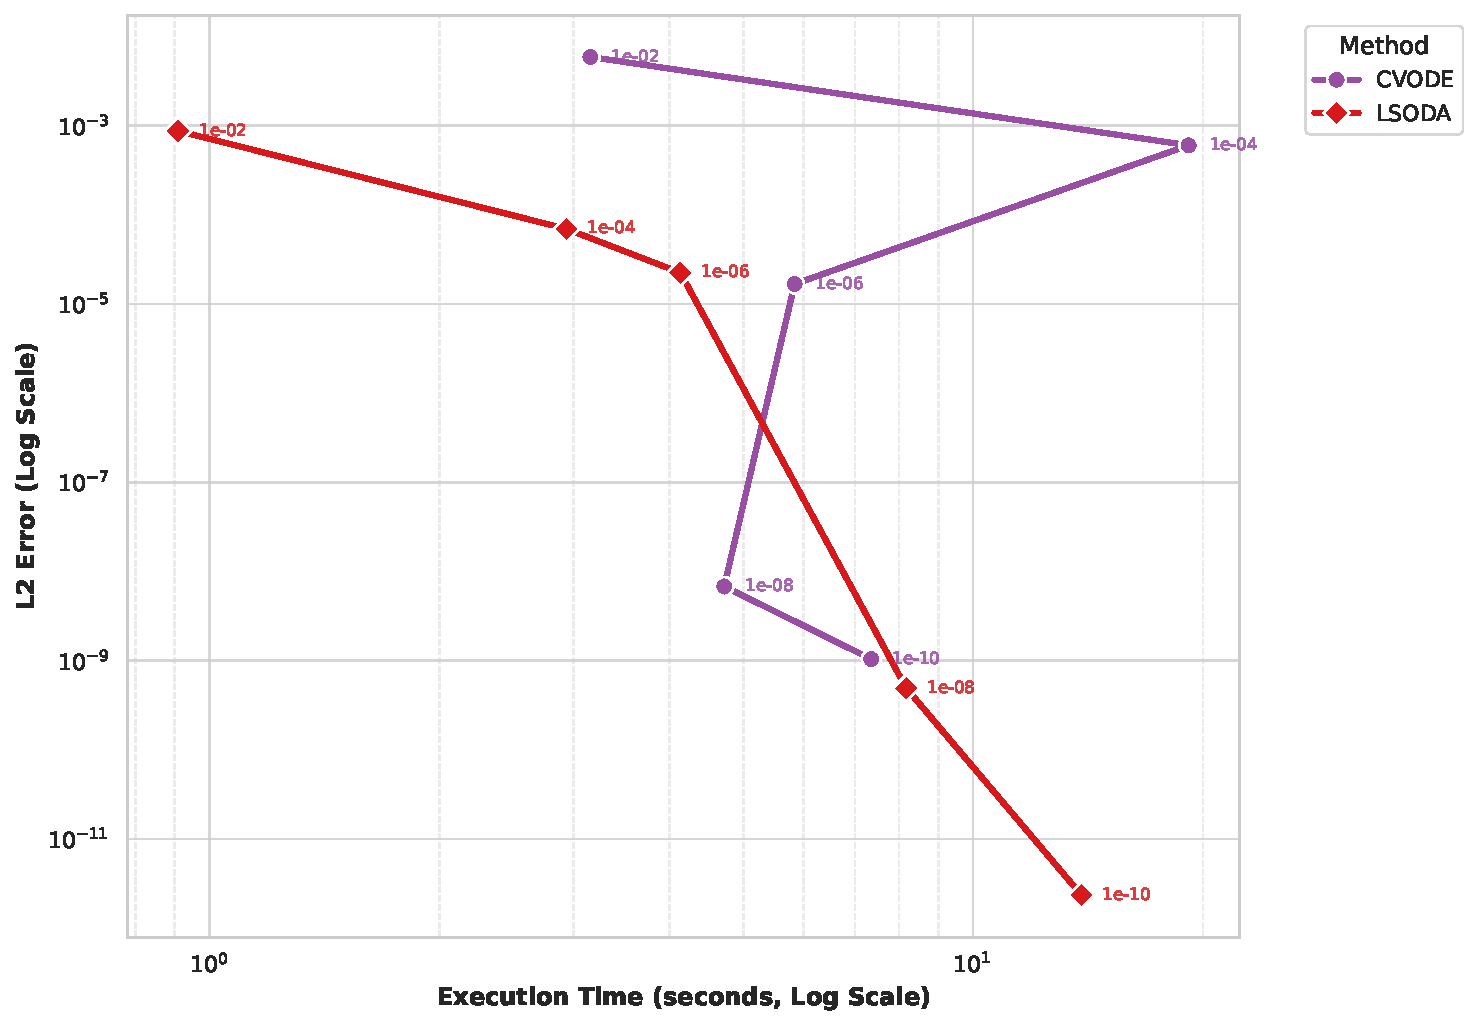
\includegraphics[width=\textwidth]{images/cvode_work_effort.pdf}
  \caption{Work-effort diagram illustrating the trade-off between \(L_2\) error and execution time for LSODA and CVODE at \(N_x = 5000\) and \(p = 3\).}
  \label{fig:cvode-work-effort}
\end{figure}
